\begin{figure}[t]
	\centering
  \begin{subfigure}{0.4\thesiswidewidth}
    \centering
    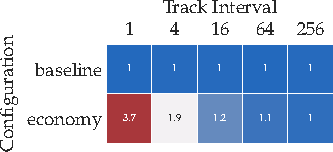
\includegraphics{../repos/cockpit-paper/fig/01_benchmark/output/fig_grid/benchmark_dummyimagenet_resnet50nobn_cuda_app_thesis-wide}
  \end{subfigure}

	\caption{\textbf{Overhead of \cockpittitle configurations on GPU for
      \resnetfifty on \imagenet.} \cockpit's instruments scale efficiently even
    to very large problems (here: $1000$ classes, $(3, 224, 224)$-sized inputs,
    and a batch size of $64$. For individual gradients to be defined, we
    replaced the batch norm layers of the \resnetfifty model with identities.)
    Color bar is the same as in \autoref{cockpit::fig:benchmark}.}
	\label{cockpit::fig:app_benchmark_configurations_gpu_imagenet}
\end{figure}

%%% Local Variables:
%%% mode: latex
%%% TeX-master: "../../../thesis"
%%% End:
